\documentclass{article}
\usepackage{polski}
\usepackage{listings}
\usepackage{graphicx}
\usepackage{xcolor}
\usepackage{float}
\usepackage{amsmath}
\newcommand{\bigO}{\mathcal{O}}

\lstdefinestyle{mystyle}{
    keywordstyle=\color{blue},       % kolor słów kluczowych
    numberstyle=\tiny\color{gray},   % kolor numerów linii
    basicstyle=\ttfamily\footnotesize, % styl podstawowy
    breaklines=true,                 % łamanie długich wierszy
    captionpos=b,                    % pozycja podpisu
    numbers=left,                    % numery linii po lewej stronie
    numbersep=1pt,                   % odstęp numerów linii
    showspaces=false,                % nie pokazuj spacji
    tabsize=2                        % rozmiar tabulacji
}

\renewcommand{\lstlistingname}{Kod}
\renewcommand{\figurename}{Wykres}

\title{Sprawozdanie - Lista 3}
\author{Jakub Zdancewicz}
\date{}

\begin{document}

\maketitle

\tableofcontents
\newpage

\section{Wstęp}
Programowanie dynamiczne to technika tworzenia algorytmów, stosowana głównie w rozwiązywaniu problemów optymalizacyjnych. Główna idea tej metody polega na podziale złożonego problemu na mniejsze, łatwiejsze do rozwiązania podproblemy, które są rozwiązywane raz, a ich wyniki przechowywane w celu uniknięcia wielokrotnego obliczania tych samych wartości. 

Podstawową zaletą programowania dynamicznego jest możliwość znaczącego skrócenia czasu działania algorytmu w porównaniu z podejściami naiwnymi, które często prowadzą do nadmiarowych obliczeń.

W niniejszym sprawozdaniu skupimy się na analizie dwóch klasycznych problemów optymalizacyjnych, które można efektywnie rozwiązać za pomocą tej techniki, oraz jednego, w którym technika programowania dynamicznego zawodzi bez zastosowania algorytmu zachłannego. Są to odpowiednio:
\begin{itemize}
    \item \textbf{Problem rozcinania pręta},
    \item \textbf{Problem znajdywania najdłuższego wspólnego podciągu},
    \item \textbf{Problem przydziału sal}.
\end{itemize}

W ramach każdego problemu przedstawimy i przeanalizujemy różnorodne podejścia do jego rozwiązania, porównując efektywność poszczególnych algorytmów na danych wejściowych o różnych rozmiarach, ze szczególnym uwzględnieniem liczby operacji przypisań, porównań oraz czasu wykonania algorytmu.
\section{Opis zaimplementowanych algorytmów}
Każdy z algorytmów został przetestowany na 10 losowo wygenerowanych ciągów danych wejściowych dla każdej z wybranych długości. Średnia liczba operacji przypisań i porównań dla $m$ ciągów o danej długości $n$ jest wyliczana według wzoru:
\[
    L_n = \sum_{i=1}^{m} \left\lceil\frac{porownania_i}{m}\right\rceil + \left\lceil\frac{przypisania_i}{m}\right\rceil
\]
gdzie:
\begin{itemize}
    \item[] $L_n$ - średnia liczba operacji dla ciągu o długości $n$,
    \item[] $\text{porownania}_i$ - liczba porównań wykonanych dla $i$-tego ciągu długości $n$,
    \item[] $\text{przypisania}_i$ - liczba przypisań wykonanych dla $i$-tego ciągu długości $n$.
\end{itemize}
Analogicznie obliczamy średni czas wykonania algorytmu dla $m$ ciągów danych wejściowych o danej długości $n$.
\subsection{Problem rozcinania pręta}
Problem rozcinania pręta polega na maksymalizacji zysku poprzez odpowiednie podzielenie pręta na fragmenty o określonych długościach. Na wejściu dany jest pręt o długości $n$ oraz tablica cen $p$ o długości $n$, gdzie $p[i]$ oznacza cenę za pręt o długości $i$. Celem jest znalezienie optymalnego sposobu podziału pręta, tak aby suma cen za jego fragmenty była maksymalna.

\subsubsection{Wersja naiwna}

Poniżej przedstawiamy naiwny algorytm rozwiązujący problem rozcinania pręta. Algorytm oparty jest na podejściu rekurencyjnym i wykorzystuje wzór na maksymalny zysk zdefiniowany jako:
\begin{equation}
   r_n = 
   \begin{cases}
   0, & \text{dla } n = 0, \\
   \max \{ p_n, \max_{i \in \{1, \dots, n-1\}} \{ p_i + r_{n-i} \} \}, & \text{dla } n > 0,
   \end{cases}
\nonumber
\end{equation}
gdzie:
\begin{itemize}
    \item $r_i$ - maksymalny zysk z pręta o długości $i$,
    \item $p_i$ - cena pręta o długości $i$.
\end{itemize}

Implementacja naiwnego algorytmu jest przedstawiona poniżej:
\begin{lstlisting}[style=mystyle, language=C++, caption={Implementacja \texttt{naive\_cut\_rod}}, label={lst:naive_cut_rod}]
int naive_cut_rod(int p[], int n)
{
    if (n == 0)
    {
        return 0;
    }
    int q = -1;
    for (int i = 1; i <= n; ++i)
    {
        q = max(q, naive_cut_rod(p, n - i) + p[i - 1]);
    }
    return q;
}
\end{lstlisting}

W tym algorytmie każdy możliwy podział pręta jest rozważany poprzez rekurencyjne wywołania dla coraz mniejszych fragmentów pręta. Niestety, algorytm ten jest skrajnie nieefektywny, ponieważ wykonuje ogromną liczbę tych samych, nadmiarowych obliczeń. Jego złożoność obliczeniowa wynosi $\Theta(2^n)$, co sprawia, że jest niepraktyczny dla dużych wartości $n$.
\subsubsection{Wersja ze spamiętywaniem}
Na szczęście, złożoność obliczeniową algorytmu można znacząco zmniejszyć, stosując technikę zapamiętywania wyników obliczeń. Zamiast wielokrotnie obliczać wynik dla tych samych podproblemów, zapamiętujemy już obliczone wartości, dzięki czemu algorytm unika nadmiarowych obliczeń.

Poniżej znajduje się implementacja algorytmu ze spamiętywaniem:
\begin{lstlisting}[style=mystyle, language=C++, caption={Implementacja \texttt{memorized\_cut\_rod}}, label={lst:memorized_cut_rod}]
int memorized_cut_rod(int p[], int r[], int s[], int n)
{
  if (r[n] >= 0)
  {
    return r[n];
  }
  int q = -1;
  if (n == 0)
  {
    q = 0;
  }
  else
  {
    for (int i = 1; i <= n; ++i)
    {
      if (q < memorized_cut_rod(p, r, s, n - i) + p[i - 1])
      {
        q = memorized_cut_rod(p, r, s, n - i) + p[i - 1];
        s[n] = i;
      }
    }
  }
  r[n] = q;
  return q;
}
\end{lstlisting}

Wersja ze spamiętywaniem opiera się na tym samym rekurencyjnym wzorze na maksymalny zysk, ale wprowadzamy dwie tablice pomocnicze:
\begin{itemize}
    \item Tablica $r$ o rozmiarze $n+1$, która przechowuje wyniki dla podproblemów, aby nie musieć ich obliczać wielokrotnie.
    \item Tablica $s$ o rozmiarze $n+1$, która zapamiętuje optymalne rozwiązania mniejszych fragmentów (rozmiary fragmentów), dzięki czemu możemy odzyskać optymalne rozwiązanie problemu.
\end{itemize}
Główna różnica w stosunku do wersji naiwnej polega na tym, że w przypadku, gdy wynik dla danego podproblemu został już obliczony, funkcja natychmiast zwraca zapisaną wartość z tablicy $r$. W przeciwnym przypadku zapisuje wynik do ponownego wykorzystania.

Dzięki zastosowaniu techniki spamiętywania, algorytm eliminuje powtarzające się obliczenia, co prowadzi do znacznego przyspieszenia działania. Złożoność obliczeniowa algorytmu spada do $\Theta (n^2)$, co jest sporym zyskiem w porównaniu do wersji naiwnej. Niestety, ponosimy dodatkowy koszt polegający na zwiększeniu złożoności pamięciowej do $\Theta (n)$, ponieważ musimy przechowywać dodatkowe tablice $r$ i $s$.
\subsubsection{Wersja iteracyjna}
Kolejną modyfikacją, jaką możemy zastosować, jest pozbycie się wywołań rekurencyjnych, zamieniając podejście rekurencyjne na podejście iteracyjne. W tym przypadku rozwiązanie problemu jest budowane krok po kroku, zaczynając od najmniejszych podproblemów (prętów o długości 0) i przechodząc aż do pełnej długości pręta $n$.
Poniżej przedstawiamy implementację podejścia iteracyjnego:
\begin{lstlisting}[style=mystyle, language=C++, caption={Implementacja \texttt{iterative\_cut\_rod}}, label={lst:iterative_cut_rod}]
void extended_bottom_up_cut_rod(int p[], int n, int r[], int s[])
{
  r[0] = 0;
  for (int j = 1; j <= n; ++j)
  {
    int q = -1;
    for (int i = 1; i <= j; ++i)
    {
      if (q < p[i - 1] + r[j - i])
      {
        q = p[i - 1] + r[j - i];
        s[j] = i;
      }
    }
    r[j] = q;
  }
}
\end{lstlisting}
W tej wersji algorytmu dla każdej długości pręta $j$ iteracyjnie obliczamy maksymalny zysk, przechodząc przez wszystkie możliwe sposoby podziału pręta (od 1 do $j$). Wzór na maksymalny zysk jest taki sam jak w wersji rekurencyjnej. W tej wersji również stosujemy technikę spamiętywania, przechowując obliczone wartości w tablicy $r$, co eliminuje powtarzające się obliczenia i przyspiesza działanie algorytmu.
Podejście iteracyjne ma złożoność obliczeniową oraz pamięciową taką samą jak podejście rekurencyjne ze spamiętywaniem.

Ponadto, w tej wersji podobnie jak w podejściu ze spamiętywaniem, zapamiętujemy optymalne rozwiązania mniejszych fragmentów pręta w tablicy $s$, co pozwala nam odzyskać optymalne rozwiązanie całego problemu.

Złożoność obliczeniowa podejścia iteracyjnego wynosi $\Theta(n^2)$, złożoność pamięciowa wynosi $\Theta(n)$. Złożoności te są takie same, jak w przypadku podejścia rekurencyjnego ze spamiętywaniem.
\subsubsection{Wyniki algorytmów}
Tabele poniżej przedstawiają wyniki eksperymentów dla algorytmów przedstawionych powyżej na danych wejściowych o różnej wielkości posortowanych rosnąco:
\begin{table}[H]
    \centering
    \scalebox{0.9}{
    \begin{tabular}{|c|c|c|c|c|}
    \hline
    \textbf{Wielkość tablicy} & \textbf{Ilość przypisań} & \textbf{Ilość porównań} & \textbf{Łączna liczba operacji} & \textbf{Czas (ms)} \\ \hline
    \textbf{2} & 10 & 9 & 19 & 0 \\ \hline
    \textbf{5} & 94 & 79 & 173 & 0 \\ \hline
    \textbf{10} & 3,070 & 2,559 & 5,629 & 0 \\ \hline
    \textbf{15} & 98,302 & 81,919 & 180,221 & 0 \\ \hline
    \textbf{20} & 3,145,726 & 2,621,439 & 5,767,165 & 9 \\ \hline
    \textbf{25} & 100,663,294 & 83,886,079 & 184,549,373 & 305 \\ \hline
    \end{tabular}
    }
    \caption{Liczba operacji i czas wykonania dla naiwnej wersji algorytmu przy różnych rozmiarach tablicy}
    \label{tab:naive_cut_rod_results}
\end{table}

\begin{table}[H]
    \centering
    \scalebox{0.9}{
    \begin{tabular}{|c|c|c|c|c|}
    \hline
    \textbf{Wielkość tablicy} & \textbf{Ilość przypisań} & \textbf{Ilość porównań} & \textbf{Łączna liczba operacji} & \textbf{Czas (ms)} \\ \hline
    \textbf{5} & 44 & 63 & 107 & 0 \\ \hline
    \textbf{10} & 113 & 200 & 313 & 0 \\ \hline
    \textbf{100} & 5,575 & 15,463 & 21,038 & 0 \\ \hline
    \textbf{1,000} & 505,918 & 1,504,710 & 2,010,628 & 2 \\ \hline
    \textbf{5,001} & 12,535,471 & 37,538,989 & 50,074,460 & 62 \\ \hline
    \textbf{10,000} & 50,059,577 & 150,047,289 & 200,106,866 & 240 \\ \hline
    \textbf{15,000} & 112,590,324 & 337,571,413 & 450,161,737 & 545 \\ \hline
    \textbf{20,000} & 200,118,834 & 600,094,418 & 800,213,252 & 1045 \\ \hline
    \end{tabular}
    }
    \caption{Liczba operacji i czas wykonania dla rekurencyjnej wersji algorytmu ze spamiętywaniem przy różnych rozmiarach tablicy}
    \label{tab:memorised_cut_rod_results}
\end{table}
\begin{table}[H]
    \centering
    \scalebox{0.9}{
    \begin{tabular}{|c|c|c|c|c|}
    \hline
    \textbf{Wielkość tablicy} & \textbf{Ilość przypisań} & \textbf{Ilość porównań} & \textbf{Łączna liczba operacji} & \textbf{Czas (ms)} \\ \hline
    \textbf{5} & 48 & 41 & 89 & 0 \\ \hline
    \textbf{10} & 122 & 131 & 253 & 0 \\ \hline
    \textbf{100} & 5,674 & 10,301 & 15,975 & 0 \\ \hline
    \textbf{1,000} & 506,917 & 1,003,001 & 1,509,918 & 1 \\ \hline
    \textbf{5,001} & 12,540,471 & 25,025,005 & 37,565,476 & 34 \\ \hline
    \textbf{10,000} & 50,069,576 & 100,030,001 & 150,099,577 & 133 \\ \hline
    \textbf{15,000} & 112,605,323 & 225,045,001 & 337,650,324 & 307 \\ \hline
    \textbf{20,000} & 200,138,833 & 400,060,001 & 600,198,834 & 565 \\ \hline
    \end{tabular}
    }
    \caption{Liczba operacji i czas wykonania dla iteracyjnej wersji algorytmu ze spamiętywaniem przy różnych rozmiarach tablicy}
    \label{tab:iterative_cut_rod_results}
\end{table}
Poniżej przedstawiamy wykresy obrazujące powyższe dane:
\begin{figure}[H]
    \centering
    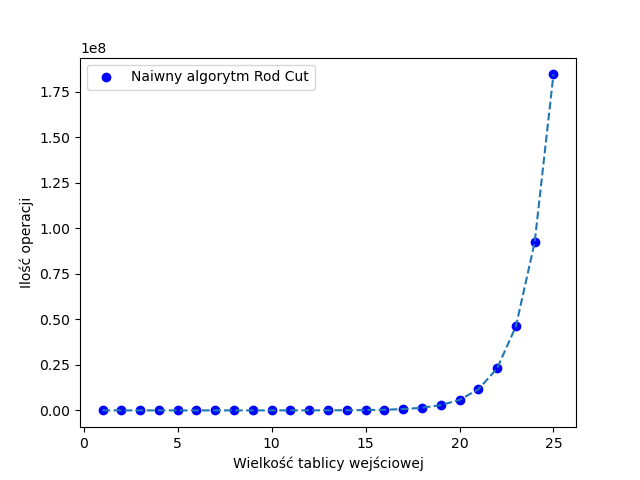
\includegraphics[width=0.8\textwidth]{Figure_1.png}
    \caption{Ilość operacji w zależności od rozmiarów danych wejściowych}
    \label{fig:naive_cut_rod}
\end{figure}
\begin{figure}[H]
    \centering
    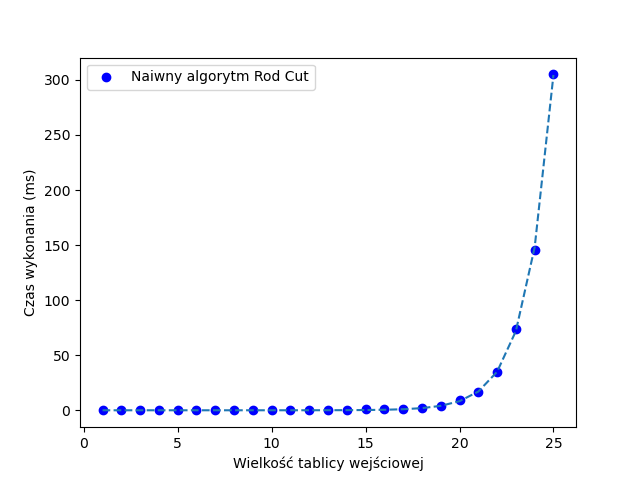
\includegraphics[width=0.8\textwidth]{Figure_3.png}
    \caption{Czas wykonania algorytmu w zależności od rozmiarów danych wejściowych}
    \label{fig:naive_cut_rodt}
\end{figure}
\begin{figure}[H]
    \centering
    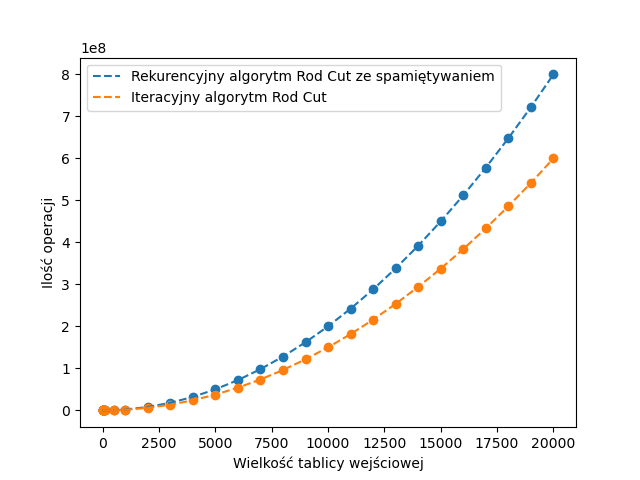
\includegraphics[width=0.8\textwidth]{Figure_2.png}
    \caption{Ilość operacji w zależności od rozmiarów danych wejściowych}
    \label{fig:mi_cut_rod}
\end{figure}
\begin{figure}[H]
    \centering
    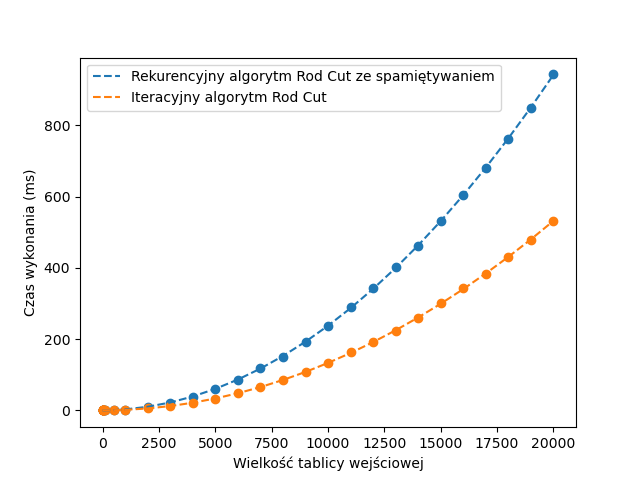
\includegraphics[width=0.8\textwidth]{Figure_4.png}
    \caption{Czas wykonania algorytmu w zależności od rozmiarów danych wejściowych}
    \label{fig:mi_cut_rodt}
\end{figure}
Niestety dla danych wejściowych o rozmiarze większym niż $20,000$ dochodzi do przepełnienia stosu w algorytmie rekurencyjnym.

Z analiz przeprowadzonych na podstawie tabel i wykresów wynika, że iteracyjny algorytm osiąga najlepsze wyniki dla dużych danych wejściowych. Jego przewaga nad wersją rekurencyjną wynika przede wszystkim z mniejszego obciążenia pamięci, ponieważ w podejściu iteracyjnym unika się kosztownego stosu wywołań funkcji charakterystycznego dla rekurencji.
\subsection{Problem znajdywania najdłuższego wspólnego podciągu}
Na wejściu dane są dwa ciągi znaków $ X = (x_1 x_2 \dots x_m) $ oraz $ Y = (y_1 y_2 \dots y_n) $. Problem polega na znalezieniu najdłuższego podciągu znaków (a właściwie jego długości), które występują w obu ciągach w tej samej kolejności.

Do rozwiązania problemu zastosujemy podejście dynamiczne oparte na rekurencyjnie zdefiniowanym wzorze:
\begin{equation}
   c[i, j] = 
   \begin{cases} 
      c[i-1, j-1] + 1, & \text{gdy } x_i = y_j, \\ 
      \max \{ c[i-1, j], c[i, j-1] \}, & \text{gdy } x_i \neq y_j,
   \end{cases}
\nonumber
\end{equation}
gdzie:
\begin{itemize}
    \item $ c[i,j] $ – długość najdłuższego wspólnego podciągu ciągów $ (x_1 x_2 \dots x_i) $ i $ (y_1 y_2 \dots y_j) $,
    \item $ x_i $ i $ y_j $ to odpowiednio $ i $-ty i $ j $-ty znak ciągów $ X $ i $ Y $.
\end{itemize}

\subsubsection{Wersja rekurencyjna ze spamiętywaniem}
Poniżej przedstawiamy implementację rekurencyjnej wersji algorytmu:

\begin{lstlisting}[style=mystyle, language=C++, caption={Implementacja \texttt{recursive\_lcs}}, label={lst:recursive_lcs}]
int recursive_lcs(string X, string Y, int m, int n, int **c, int **b) {
  if (c[m][n] != -1) {
    return c[m][n];
  }
  if (m == 0 || n == 0) {
    c[m][n] = 0;
    return c[m][n];
  }
  if (X[m - 1] == Y[n - 1]) {
    c[m][n] = recursive_lcs(X, Y, m - 1, n - 1, c, b) + 1;
    b[m][n] = 3;
    return c[m][n];
  }
  if (recursive_lcs(X, Y, m - 1, n, c, b) < recursive_lcs(X, Y, m, n - 1, c, b)) {
    c[m][n] = recursive_lcs(X, Y, m, n - 1, c, b);
    b[m][n] = 1;
  } else {
    c[m][n] = recursive_lcs(X, Y, m - 1, n, c, b);
    b[m][n] = 2;
  }
  return c[m][n];
}
\end{lstlisting}

Rekurencyjna wersja algorytmu opiera się na obliczaniu wartości w tablicy $c$ poprzez rekurencyjne wywołania funkcji \texttt{recursive\_lcs()}, które stosują wzór zaprezentowany powyżej. Algorytm korzysta również z dodatkowej tablicy $b$, która przechowuje informacje o kierunkach (3 – ukośnie, 2 – w górę, 1 – w lewo). Te informacje są później wykorzystywane do odtworzenia najdłuższego wspólnego podciągu. 

Każde wywołanie funkcji sprawdza, czy dla danej pary indeksów $i$ i $j$ wartość w tablicy $c[i][j]$ została już obliczona. Jeśli tak, funkcja zwraca jej wartość, co pozwala uniknąć powtarzania obliczeń.

Dzięki takiemu podejściu algorytm działa w czasie $O(m \cdot n)$, gdzie $m$ i $n$ to długości ciągów $X$ i $Y$, a także wymaga $O(m \cdot n)$ pamięci na przechowanie tablic $c$ i $b$.

\subsubsection{Wersja iteracyjna ze spamiętywaniem}
Poniżej przedstawiamy implementację iteracyjnej wersji algorytmu:
\begin{lstlisting}[style=mystyle, language=C++, caption={Implementacja \texttt{iterative\_lcs}}, label={lst:iterative_lcs}]
void iterative_lcs(string X, string Y, int m, int n, int **c, int **b)
{
  for (int i = 1; i <= m; ++i)
  {
    for (int j = 1; j <= n; ++j)
    {
      if (X[i - 1] == Y[j - 1])
      {
        c[i][j] = c[i - 1][j - 1] + 1;
        b[i][j] = 3;
      }
      else if (c[i - 1][j] >= c[i][j - 1])
      {
        c[i][j] = c[i - 1][j];
        b[i][j] = 2;
      }
      else
      {
        c[i][j] = c[i][j - 1];
        b[i][j] = 1;
      }
    }
  }
}
\end{lstlisting}
Iteracyjna wersja algorytmu również opiera się na powyższym wzorze. Jedyną różnicą w stosunku do wersji rekurencyjnej jest to, że tablica $c$ jest wypełniana iteracyjnie od początku, a nie od końca przez rekurencyjne wywołania funkcji. Dzięki temu unikamy kosztów związanych z wieloma wywołaniami funkcji rekurencyjnych.

Podobnie jak w wersji rekurencyjnej, w iteracyjnej wersji algorytmu używamy tablicy $b$, która przechowuje informacje o kierunkach (3 – ukośnie, 2 – w górę, 1 – w lewo). Te informacje pozwalają na późniejsze odtworzenie najdłuższego wspólnego podciągu.

Algorytm iteracyjny, podobnie jak rekurencyjny, działa w czasie $O(m \cdot n)$ i ma złożoność pamięciową $O(m \cdot n)$, gdzie $m$ i $n$ to długości ciągów $X$ i $Y$.
\subsubsection{Odzyskiwanie rozwiązania}
Poniżej przedstawiamy implementację kodu służącego do odzyskania rozwiązania problemu najdłuższego wspólnego podciągu:
\begin{lstlisting}[style=mystyle, language=C++, caption={Implementacja \texttt{print\_lcs\_solution}}, label={lst:print_lcs_solution}]
void print_lcs_solution(string X, int **b, int m, int n)
{
  if (m == 0 || n == 0)
  {
    return;
  }
  if (b[m][n] == 3)
  {
    print_lcs_solution(X, b, m - 1, n - 1);
    cout << X[m - 1];
  }
  else if (b[m][n] == 2)
  {
    print_lcs_solution(X, b, m - 1, n);
  }
  else if (b[m][n] == 1)
  {
    print_lcs_solution(X, b, m, n - 1);
  }
}
\end{lstlisting}
Odzyskiwanie rozwiązania polega na poruszaniu się po tablicy $b$ w odwrotnej kolejności, zaczynając od komórki $b[m][n]$. Wartości w tablicy $b$ wskazują kierunki, w jakich należy przejść, aby odtworzyć najdłuższy wspólny podciąg. Jeśli wartość $b[m][n]$ wynosi 3, oznacza to, że znak na pozycji $m-1$ w ciągu $X$ jest częścią najdłuższego wspólnego podciągu, więc wypisujemy ten znak i przechodzimy "na skos" do komórki $b[m-1][n-1]$. Jeśli wartość $b[m][n]$ wynosi 2, oznacza to, że musimy przejść do góry, czyli do komórki $b[m-1][n]$. Z kolei wartość 1 w tablicy $b$ wskazuje, że należy przejść w lewo, do komórki $b[m][n-1]$. 

Proces ten jest rekurencyjny i powtarza się, aż dotrzemy do krawędzi tablicy, gdzie jeden z indeksów $m$ lub $n$ wynosi 0, co kończy odtwarzanie podciągu.
\subsubsection{Wyniki algorytmów}
Tabele poniżej przedstawiają wyniki eksperymentów dla algorytmów przedstawionych powyżej na danych wejściowych o różnej wielkości:
\begin{table}[H]
    \centering
    \scalebox{0.9}{
    \begin{tabular}{|c|c|c|c|c|}
    \hline
    \textbf{Wielkość tablicy} & \textbf{Ilość przypisań} & \textbf{Ilość porównań} & \textbf{Łączna liczba operacji} & \textbf{Czas (ms)} \\ \hline
    \textbf{5} & 57 & 158 & 215 & 0 \\ \hline
    \textbf{50} & 4,941 & 14,536 & 19,477 & 1 \\ \hline
    \textbf{101} & 19,798 & 58,433 & 78,231 & 3 \\ \hline
    \textbf{500} & 480,754 & 1,422,842 & 1,903,596 & 113 \\ \hline
    \textbf{1000} & 1,922,658 & 5,692,158 & 7,614,816 & 650 \\ \hline
    \textbf{1500} & 4,314,811 & 12,775,312 & 17,090,123 & 1375 \\ \hline
    \textbf{2201} & 9,321,120 & 27,600,400 & 36,921,520 & 3715 \\ \hline
    \textbf{3000} & 17,294,530 & 51,211,141 & 68,505,671 & 8094 \\ \hline
    \end{tabular}
    }
    \caption{Liczba operacji i czas wykonania dla rekurencyjnej wersji algorytmu przy różnych rozmiarach tablicy}
    \label{tab:recursive_lcs}
\end{table}

\begin{table}[H]
    \centering
    \scalebox{0.9}{
    \begin{tabular}{|c|c|c|c|c|}
    \hline
    \textbf{Wielkość tablicy} & \textbf{Ilość przypisań} & \textbf{Ilość porównań} & \textbf{Łączna liczba operacji} & \textbf{Czas (ms)} \\ \hline
    \textbf{5} & 86 & 85 & 171 & 0 \\ \hline
    \textbf{50} & 7,601 & 7,502 & 15,103 & 0 \\ \hline
    \textbf{101} & 30,806 & 30,406 & 61,212 & 0 \\ \hline
    \textbf{500} & 751,001 & 741,385 & 1,492,386 & 2 \\ \hline
    \textbf{1000} & 3,002,001 & 2,963,531 & 5,965,532 & 10 \\ \hline
    \textbf{1500} & 6,753,001 & 6,666,333 & 13,419,334 & 17 \\ \hline
    \textbf{2201} & 14,537,606 & 14,351,299 & 28,888,905 & 39 \\ \hline
    \textbf{3000} & 27,006,001 & 26,659,373 & 53,665,374 & 71 \\ \hline
    \end{tabular}
    }
    \caption{Liczba operacji i czas wykonania dla iteracyjnej wersji algorytmu przy różnych rozmiarach tablicy}
    \label{tab:iterative_lcs}
\end{table}
\begin{figure}[H]
    \centering
    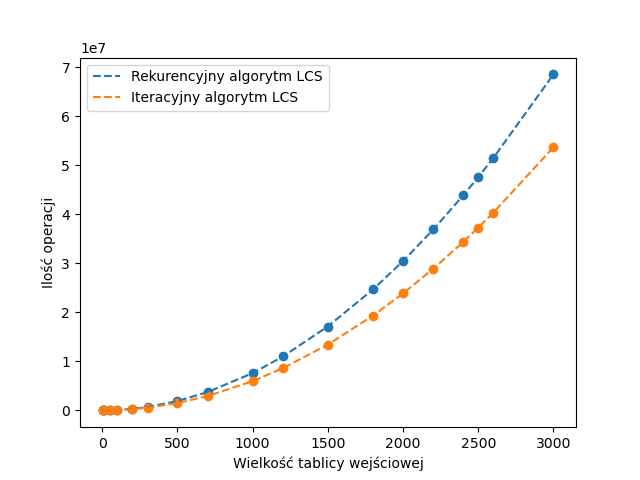
\includegraphics[width=0.8\textwidth]{Figure_5.png}
    \caption{Ilość operacji w zależności od rozmiarów danych wejściowych}
    \label{fig:lcs}
\end{figure}
\begin{figure}[H]
    \centering
    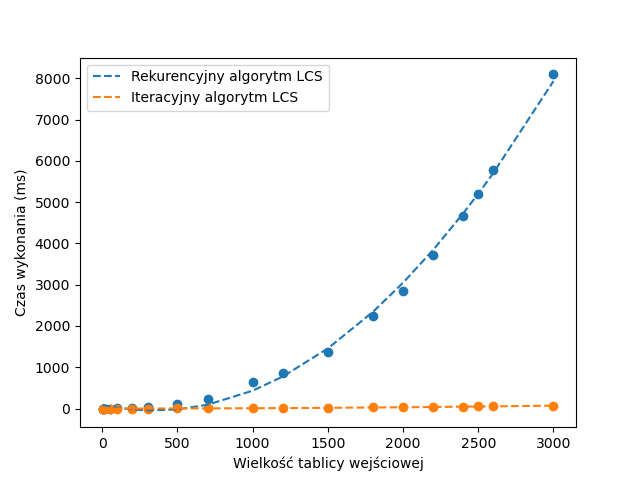
\includegraphics[width=0.8\textwidth]{Figure_6.png}
    \caption{Czas wykonania w zależności od rozmiarów danych wejściowych}
    \label{fig:lcs}
\end{figure}
Jak wynika z wykresów i tabeli, wersja rekurencyjna jest dużo wolniejsza od wersji iteracyjnej, mimo że wykonuje przybliżoną ilość operacji.
\subsection{Problem przydziału sal}
Dane są następujące elementy:
\begin{itemize}
    \item Jedna sala (zasób), którą można wykorzystać do organizacji wydarzeń.
    \item $n$ wydarzeń, z których każde jest określone przez przedział czasowy $[s_i, f_i)$, gdzie $0 \leq s_i < f_i < \infty$ dla $i = 1, 2, \dots, n$.
\end{itemize}

Celem jest znalezienie możliwie największego zbioru wydarzeń, które nie nakładają się na siebie w czasie. Zakładamy, że wydarzenia są posortowane rosnąco względem czasu zakończenia, tj. $f_1 \leq f_2 \leq \dots \leq f_n$.

Nasze pierwsze rozwiązanie, oparte na programowaniu dynamicznym, zostało zaimplementowane na podstawie rekurencyjnie zdefiniowanego wzoru:

\begin{equation}
   c[i, j] = 
   \begin{cases} 
      0, & \text{jeśli } S_{ij} = \emptyset, \\ 
      \max \left\{ c[i, k] + c[k, j] + 1 : k \in S_{ij} \right\}, & \text{jeśli } S_{ij} \neq \emptyset,
   \end{cases}
\nonumber
\end{equation}

gdzie:
\begin{itemize}
    \item $ S_{ij} $ – zbiór wydarzeń, które rozpoczynają się po zakończeniu $i$-tego wydarzenia i kończą się przed rozpoczęciem $j$-tego wydarzenia,
    \item $c[i,j]$ – maksymalna liczba wzajemnie niekolidujących wydarzeń z $S_{ij}$.
\end{itemize}

Dodatkowo przedstawimy rozwiązanie oparte na algorytmie zachłannym, które w każdym kroku wybiera najbardziej optymalne wydarzenie, czyli takie, które rozpoczyna się jak najwcześniej i nie koliduje z wcześniej wybranymi wydarzeniami. 

Niech $S_k = \{ m : s[m] \geq f[k] \}$ będzie zbiorem zadań, które rozpoczynają się po zakończeniu $k$-tego zadania.

Można wykazać, że optymalne rozwiązanie problemu doboru sal dla zbioru $S_k$ zawiera zadanie $\min S_k$, czyli zadanie, które ma najwcześniejszy czas zakończenia spośród wszystkich zadań w zbiorze $S_k$. Co udowadnia, że algorytm zachłanny jest poprawnym algorytmem dla tego problemu.

W każdym z przedstawionych poniżej algorytmów wydarzenia przechowywujemy w strukturze danych zaimplementowanej w następujący sposób:
\begin{lstlisting}[style=mystyle, language=C++, caption={Implementacja \texttt{activity}}, label={lst:activity}]
struct Activity
{
  int start;
  int end;
};
\end{lstlisting}

\subsubsection{Wersja oparta na programowaniu dynamicznym}
Poniżej przedstawiamy implementację algorytmu rozwiązującego problem przydziału sal przy pomocy programowania dynamicznego:
\begin{lstlisting}[style=mystyle, language=C++, caption={Implementacja \texttt{dp\_activity\_selector}}, label={lst:dp_activity_selector}]
int dp_activity_selector(Activity activities[], int n, int **c, int **act) {
  for (int i = 0; i <= n + 1; ++i) {
    for (int j = 0; j <= n + 1; ++j) {
      c[i][j] = 0;
      act[i][j] = -1;
    }
  }
  for (int l = 2; l <= n + 1; ++l) {
    for (int i = 0; i <= n + 1 - l; ++i)
    {
      int j = i + l;
      c[i][j] = 0;
      for (int k = i + 1; k < j; ++k)
      {
        if (activities[i].end <= activities[k].start && activities[k].end <= activities[j].start && c[i][k] + c[k][j] + 1 > c[i][j])
        {
          c[i][j] = c[i][k] + c[k][j] + 1;
          act[i][j] = k;
        }
      }
    }
  }
  return c[0][n + 1];
}
\end{lstlisting}
W tej wersji algorytmu korzystamy z dwuwymiarowej tablicy $c[i][j]$, w której przechowujemy maksymalną liczbę wzajemnie niekolidujących wydarzeń pomiędzy wydarzeniami $i$ i $j$, oraz tablicy $act[i][j]$, która przechowuje indeksy wybranych wydarzeń, co pozwala później na odzyskanie rozwiązania. 

Algorytm iteruje po kolejnych długościach przedziałów czasowych $[i, j]$, rozpoczynając od przedziałów o długości 2. Następnie, dla każdego przedziału $[i, j]$, algorytm wypełnia tablicę $c$ zgodnie z rekurencyjnym wzorem podanym powyżej, używając wartości dla krótszych przedziałów czasowych, które zostały obliczone w poprzednich krokach pętli.

Zasadniczo, dla każdej pary przedziałów $[i, j]$, algorytm stara się znaleźć takie wydarzenie $k$ (gdzie $i < k < j$), które może zostać wybrane do rozwiązania, zapewniając, że wydarzenia $i$, $k$ i $j$ są wzajemnie niekolidujące.

Złożoność obliczeniowa tego algorytmu wynosi $\Theta(n^3)$, ponieważ dla każdego przedziału $[i, j]$ algorytm iteruje po wszystkich możliwych wartościach $k$ w tym przedziale. Złożoność pamięciowa tego algorytmu wynosi $\bigO(n^2)$
\subsubsection{Zachłanna wersja rekurencyjna}
Poniżej przedstawiamy implementację zachłannej wersji rekurencyjnego algorytmu rozwiązującego problem przydziału sal:
\begin{lstlisting}[style=mystyle, language=C++, caption={Implementacja \texttt{greedy\_recursive\_activity\_selector}}, label={lst:recursive_activity_selector}]
void recursive_activity_selector(Activity activities[], int n, int k, Activity selected[], int &selected_count)
{
  int m = k + 1;
  while (m < n && activities[m].start < activities[k].end)
  {
    m++;
  }
  if (m < n)
  {
    selected[selected_count++] = activities[m];
    recursive_activity_selector(activities, n, m, selected, selected_count);
  }
}
\end{lstlisting}
Algorytm polega na zachłannym wyborze zadania o najwcześniejszym zakończeniu. Dzięki temu, w każdym kroku algorytmu, wybieramy zadanie, które kończy się najwcześniej, co pozwala na maksymalne wykorzystanie dostępnego czasu i umożliwia wybór jak największej liczby niekolidujących zadań.

Dodatkowo, w algorytmie implementujemy tablicę $selected[]$, która służy do zapisywania wybranych zadań. Tablica ta pozwala nam później łatwo odzyskać optymalne rozwiązanie.

Złożoność obliczeniowa tego algorytmu wynosi $\Theta(n-k+1)$, złożoność pamięciowa tego algorytmu wynosi $\bigO(n)$.
\subsubsection{Zachłanna wersja iteracyjna}
Poniżej przedstawiamy implementację zachłannej wersji iteracyjnego algorytmu rozwiązującego problem przydziału sal:

\begin{lstlisting}[style=mystyle, language=C++, caption={Implementacja \texttt{greedy\_iterative\_activity\_selector}}, label={lst:iterative_activity_selector}]
int iterative_activity_selector(Activity activities[], int n, Activity selected[])
{
  int k = 0;
  selected[0] = activities[k];
  int selected_count = 1;
  for (int m = 1; m < n; ++m)
  {
    if (activities[m].start >= activities[k].end)
    {
      selected[selected_count++] = activities[m];
      k = m;
    }
  }
  return selected_count;
}
\end{lstlisting}
Algorytm iteracyjny jest praktycznie identyczny w porównaniu do algorytmu rekurencyjnego. Zrezygnowanie z rekurencji pozwala na zmniejszenie obciążenia stosu wywołań, co umożliwia używanie algorytmu dla większych danych wejściowych.

Podsumowując, różnica między wersją rekurencyjną a iteracyjną polega głównie na sposobie realizacji algorytmu, co wpływa na efektywność zarządzania pamięcią, a nie na złożoność obliczeniową czy pamięciową, która jest równa złożoności wersji rekurencyjnej w obu przypadkach.
\subsubsection{Modyfikacja algorytmu}
Poniżej przedstawiamy implementację zmodyfikowanej iteracyjnej wersji algorytmu, która umożliwia zastosowanie algorytmu do danych posortowanych względem czasu rozpoczęcia wydarzenia:
\begin{lstlisting}[style=mystyle, language=C++, caption={Implementacja \texttt{modified\_greedy\_iterative\_activity\_selector}}, label={lst:modified_iterative_activity_selector}]
int modified_activity_selector(Activity activities[], int n, Activity selected[]) {
  int k = n - 1;
  selected[0] = activities[k];
  int selected_count = 1;
  for (int m = n - 2; m > -1; --m)
  {
    if (activities[m].end <= activities[k].start)
    {
      selected[selected_count++] = activities[m];
      k = m;
    }
  }
  return selected_count;
}
\end{lstlisting}
Główną ideą działania tego algorytmu jest iteracja po tablicy wydarzeń od tyłu. Dzięki temu, mimo że dane są posortowane względem czasu rozpoczęcia wydarzeń, algorytm może je przetwarzać w sposób kompatybilny ze zwykłym algorytmem zachłannym, który wymaga, by dane były posortowane według czasów zakończenia wydarzeń. Algorytm działa wtedy identycznie jak ten przedstawiony wcześniej.

Takie podejście umożliwia zachowanie niezmienionej liczby wybranych wydarzeń, a zmienia jedynie kolejność ich przetwarzania. W rezultacie algorytm działa tak samo, jak tradycyjny algorytm zachłanny, ale na danych posortowanych według czasów rozpoczęcia.
\subsubsection{Wyniki algorytmów}
Tabele poniżej przedstawiają wyniki eksperymentów dla algorytmów przedstawionych powyżej na danych wejściowych o różnej wielkości posortowanych rosnąco według zakończeń:
\begin{table}[H]
    \centering
    \scalebox{0.9}{
    \begin{tabular}{|c|c|c|c|c|}
    \hline
    \textbf{Wielkość tablicy} & \textbf{Ilość przypisań} & \textbf{Ilość porównań} & \textbf{Łączna liczba operacji} & \textbf{Czas (ms)} \\ \hline
    \textbf{5} & 270 & 240 & 510 & 0 \\ \hline
    \textbf{10} & 927 & 1170 & 2097 & 0 \\ \hline
    \textbf{107} & 277,763 & 863,500 & 1,141,263 & 2 \\ \hline
    \textbf{309} & 5,534,556 & 20,053,904 & 25,588,460 & 30 \\ \hline
    \textbf{505} & 23,117,022 & 86,883,240 & 110,000,262 & 130 \\ \hline
    \textbf{750} & 73,960,779 & 283,507,010 & 357,467,789 & 434 \\ \hline
    \textbf{1000} & 173,155,742 & 670,676,010 & 843,831,752 & 1098 \\ \hline
    \end{tabular}
    }
    \caption{Liczba operacji i czas wykonania dla wersji algorytmu opartej na programowaniu dynamicznym przy różnych rozmiarach tablicy}
    \label{tab:dp_activity_selector}
\end{table}
\begin{table}[H]
    \centering
    \scalebox{0.9}{
    \begin{tabular}{|c|c|c|c|c|}
    \hline
    \textbf{Wielkość tablicy} & \textbf{Ilość przypisań} & \textbf{Ilość porównań} & \textbf{Łączna liczba operacji} & \textbf{Czas (ms)} \\ \hline
    \textbf{5} & 6 & 12 & 18 & 0 \\ \hline
    \textbf{50} & 58 & 109 & 167 & 0 \\ \hline
    \textbf{501} & 592 & 1,094 & 1,686 & 0 \\ \hline
    \textbf{1000} & 1,176 & 2,177 & 3,353 & 0 \\ \hline
    \textbf{5001} & 5,889 & 10,891 & 16,780 & 0 \\ \hline
    \textbf{10000} & 11,780 & 21,781 & 33,561 & 1 \\ \hline
    \textbf{40001} & 47,092 & 87,094 & 134,186 & 1 \\ \hline
    \textbf{65000} & 76,488 & 141,489 & 217,977 & 2 \\ \hline
    \end{tabular}
    }
    \caption{Liczba operacji i czas wykonania dla rekurencyjnej wersji zachłannego algorytmu przy różnych rozmiarach tablicy}
    \label{tab:recursive_activity_selector}
\end{table}
\begin{table}[H]
    \centering
    \scalebox{0.9}{
    \begin{tabular}{|c|c|c|c|c|}
    \hline
    \textbf{Wielkość tablicy} & \textbf{Ilość przypisań} & \textbf{Ilość porównań} & \textbf{Łączna liczba operacji} & \textbf{Czas (ms)} \\ \hline
    \textbf{5} & 9 & 9 & 18 & 0 \\ \hline
    \textbf{50} & 69 & 99 & 168 & 0 \\ \hline
    \textbf{501} & 685 & 1,001 & 1,686 & 0 \\ \hline
    \textbf{1000} & 1,355 & 1,999 & 3,354 & 0 \\ \hline
    \textbf{5001} & 6,779 & 10,001 & 16,780 & 0 \\ \hline
    \textbf{10000} & 13,563 & 19,999 & 33,562 & 0 \\ \hline
    \textbf{40001} & 54,186 & 80,001 & 134,187 & 0 \\ \hline
    \textbf{65000} & 87,979 & 129,999 & 217,978 & 1 \\ \hline
    \end{tabular}
    }
    \caption{Liczba operacji i czas wykonania dla iteracyjnej wersji zachłannego algorytmu przy różnych rozmiarach tablicy}
    \label{tab:iterative_activity_selector}
\end{table}
\begin{figure}[H]
    \centering
    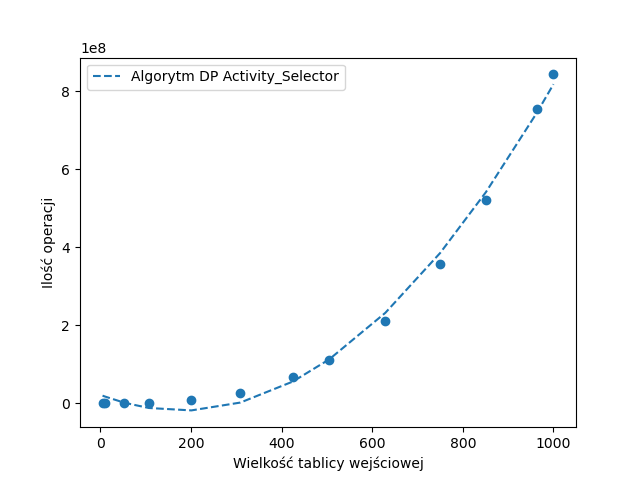
\includegraphics[width=0.7\textwidth]{Figure_7.png}
    \caption{Ilość operacji w zależności od rozmiarów danych wejściowych}
    \label{fig:das}
\end{figure}
\begin{figure}[H]
    \centering
    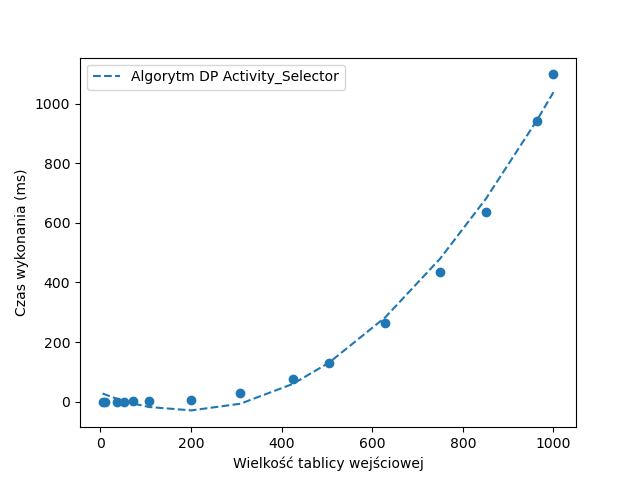
\includegraphics[width=0.7\textwidth]{Figure_9.png}
    \caption{Czas wykonania w zależności od rozmiarów danych wejściowych}
    \label{fig:das}
\end{figure}
\begin{figure}[H]
    \centering
    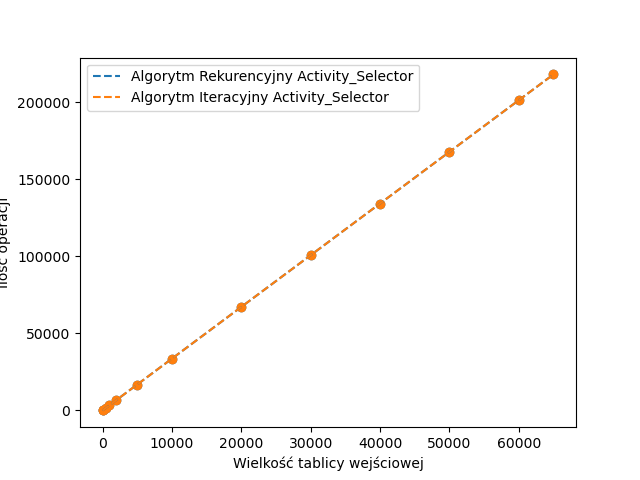
\includegraphics[width=0.7\textwidth]{Figure_8.png}
    \caption{Ilość operacji w zależności od rozmiarów danych wejściowych}
    \label{fig:as}
\end{figure}
Z tabel i wykresów jednoznacznie wynika, że algorytm oparty na programowaniu dynamicznym jest znacznie wolniejszy od obu wersji algorytmów zachłannych, które natomiast wykonują niemal identyczną liczbę operacji. Niestety, algorytm rekurencyjny przepełnia stos przy rozmiarze przekraczającym $65,000$.
\section{Wnioski}

Analiza zaimplementowanych algorytmów pozwala na wyciągnięcie następujących wniosków:

\begin{enumerate}
    \item Algorytm \texttt{CUT\_ROD}:
    \begin{itemize}
        \item Wersja naiwna charakteryzuje się bardzo dużą liczbą wywołań rekurencyjnych, co prowadzi do znacznego wydłużenia czasu działania dla większych danych wejściowych.
        \item Wersja rekurencyjna ze spamiętaniem znacznie skraca czas wykonania, eliminując konieczność wielokrotnego obliczania tych samych podproblemów. Niestety, dla dużych danych pojawia się problem przepełnienia stosu.
        \item Wersja iteracyjna jest szybsza od wersji rekurencyjnej i odporna na problem przepełnienia stosu.
    \end{itemize}

    \item Algorytm \texttt{LCS}:
    \begin{itemize}
        \item Wersja rekurencyjna dobrze radzi sobie dla małych danych, jednak przy większych rozmiarach zauważalnie odstaje od wersji iteracyjnej, a dodatkowo pojawia się problem przepełnienia stosu.
        \item Wersja iteracyjna jest najbardziej efektywna zarówno pod względem czasu, jak i pamięci, co czyni ją preferowaną opcją w praktycznych zastosowaniach.
    \end{itemize}

    \item Algorytm \texttt{ACTIVITY\_SELECTOR}:
    \begin{itemize}
        \item Wersja iteracyjna okazała się bardziej efektywna niż rekurencyjna, eliminując problem przepełnienia stosu. Dla małych danych obie wersje wykazują niemal identyczne działanie.
        \item Algorytm oparty na programowaniu dynamicznym jest nieoptymalny dla tego problemu, szczególnie dla większych danych wejściowych, gdzie podejście zachłanne daje lepsze wyniki.
    \end{itemize}

    \item Najważniejsze wnioski:
    \begin{itemize}
        \item Wykorzystanie programowania dynamicznego i techniki spamiętywania wyników może znacznie poprawić efektywność algorytmów w porównaniu do wersji naiwnych.
        \item Wersje rekurencyjne są podatne na problem przepełnienia stosu, co ogranicza ich zastosowanie do relatywnie małych danych wejściowych.
        \item Podejście zachłanne, jeśli jest poprawne w kontekście danego problemu, może znacznie zmniejszyć złożoność obliczeniową i poprawić efektywność działania.
        \item Iteracyjne wersje algorytmów eliminują problemy związane z przepełnieniem stosu.
    \end{itemize}
\end{enumerate}
\end{document}
